%%%%%%%%%%%%%%%%%%%%%%%%%%%%%%%%%%%%%%%%%%%%%%%%%%%%%%%%%%%%%%%%%%%%%%%%%%%%%%%%
%2345678901234567890123456789012345678901234567890123456789012345678901234567890
%        1         2         3         4         5         6         7         8

\documentclass[letterpaper, 10 pt, conference]{ieeeconf}  % Comment this line out if you need a4paper

%\documentclass[a4paper, 10pt, conference]{ieeeconf}      % Use this line for a4 paper

\IEEEoverridecommandlockouts                              % This command is only needed if 
                                                          % you want to use the \thanks command

\overrideIEEEmargins                                      % Needed to meet printer requirements.

% Added from SE since LaTeX recognises everything in UTF-8 and otherwise this has to be mentioned
\UseRawInputEncoding

%In case you encounter the following error:
%Error 1010 The PDF file may be corrupt (unable to open PDF file) OR
%Error 1000 An error occurred while parsing a contents stream. Unable to analyze the PDF file.
%This is a known problem with pdfLaTeX conversion filter. The file cannot be opened with acrobat reader
%Please use one of the alternatives below to circumvent this error by uncommenting one or the other
%\pdfobjcompresslevel=0
%\pdfminorversion=4

% See the \addtolength command later in the file to balance the column lengths
% on the last page of the document

% The following packages can be found on http:\\www.ctan.org
%\usepackage{graphics} % for pdf, bitmapped graphics files
%\usepackage{epsfig} % for postscript graphics files
%\usepackage{mathptmx} % assumes new font selection scheme installed
%\usepackage{times} % assumes new font selection scheme installed
%\usepackage{amsmath} % assumes amsmath package installed
%\usepackage{amssymb}  % assumes amsmath package installed

% Helpful commands from insti papers
% Packages
\usepackage{xspace}
\usepackage{graphicx}
\usepackage{xcolor}
% Comments
\newcommand{\asc}[1]{{\color{blue!50!black} [Sat: {\em #1}]}\xspace}
\newcommand{\tbd}[1]{{\color{red!100!black} [TBD: {\em #1}]}\xspace}
% Citation
\newcommand{\mlabel}[1]{\textrm{ \color{blue} (#1) }\label{#1}}
\newcommand{\mcite}[1]{\cite{#1}\textrm{\color{blue}(\texttt{\detokenize{#1}})}}
\newcommand{\mref}[1]{\ref{#1}\textrm{\color{blue}(#1)}}
% Paths
\graphicspath{{./graphics/}}

\title{\LARGE \bf
Computational robust co-design for the top-down development of a humanoid robot arm \\
\asc{Started: 07-06-2022}
}


\author{Albert Author$^{1}$ and Bernard D. Researcher$^{2}$% <-this % stops a space
\thanks{*This work was not supported by any organization}% <-this % stops a space
\thanks{$^{1}$Albert Author is with Faculty of Electrical Engineering, Mathematics and Computer Science,
        University of Twente, 7500 AE Enschede, The Netherlands
        {\tt\small albert.author@papercept.net}}%
\thanks{$^{2}$Bernard D. Researcheris with the Department of Electrical Engineering, Wright State University,
        Dayton, OH 45435, USA
        {\tt\small b.d.researcher@ieee.org}}%
}


\begin{document}

\maketitle
\thispagestyle{empty}
\pagestyle{empty}


%%%%%%%%%%%%%%%%%%%%%%%%%%%%%%%%%%%%%%%%%%%%%%%%%%%%%%%%%%%%%%%%%%%%%%%%%%%%%%%%
\begin{abstract}
The paper presents a top-down development of a humanoid robot arm, via computational design. Unlike point based designs resulting from a conventional optimisation algorithm, the proposed method offers a range of values for the design variables within which the design is still feasible with respect to the chosen requirements. The design procedure includes simultaneous optimisation of both the mechanical, control  and hardware parameters to identify the optimal design with respect to a task. We propose a novel framework involving classical optimisation followed by obtaining solution spaces for various design variables to identify a robust design. Moreover, to emphasize the need for physically feasible designs, we show that designers could exploit the later step to trade-off different design variables across mechanical, control or hardware parameters, for cost, manufacturability, style, behavior of the robot etc. The robot arm constructed following the proposed approach not only consumes lesser energy for the motion and is aptly sized for a range of tasks involving general table-top assembly tasks. \asc{Define tasks as a class of tasks from the NIST board, without actually talking about the NIST board}. 
\end{abstract}


%%%%%%%%%%%%%%%%%%%%%%%%%%%%%%%%%%%%%%%%%%%%%%%%%%%%%%%%%%%%%%%%%%%%%%%%%%%%%%%%
\section{INTRODUCTION}
Paper structure follows the previous work,~\mcite{fadini_computational_2021}.
\asc{The argument could be that we have a lot of table-top tasks and somehow, we use overdesigned robots to solve simple pick and fix kinda tasks and we want to make a robot that is rightly sized for this task and like tasks.}

\section{METHODOLOGY}

\subsection{Requirements definition and the problem solving procedure}
\asc{Includes requirements, motivation from the NIST board, ADGs, XDSMs, etc.}
\tbd{Add an inbuilt table for requirements}
\tbd{Both of the ADG and XDSM needs changing to the actual form of scope of the project--> Include structures or not}
\begin{figure}[h]
	\centering
	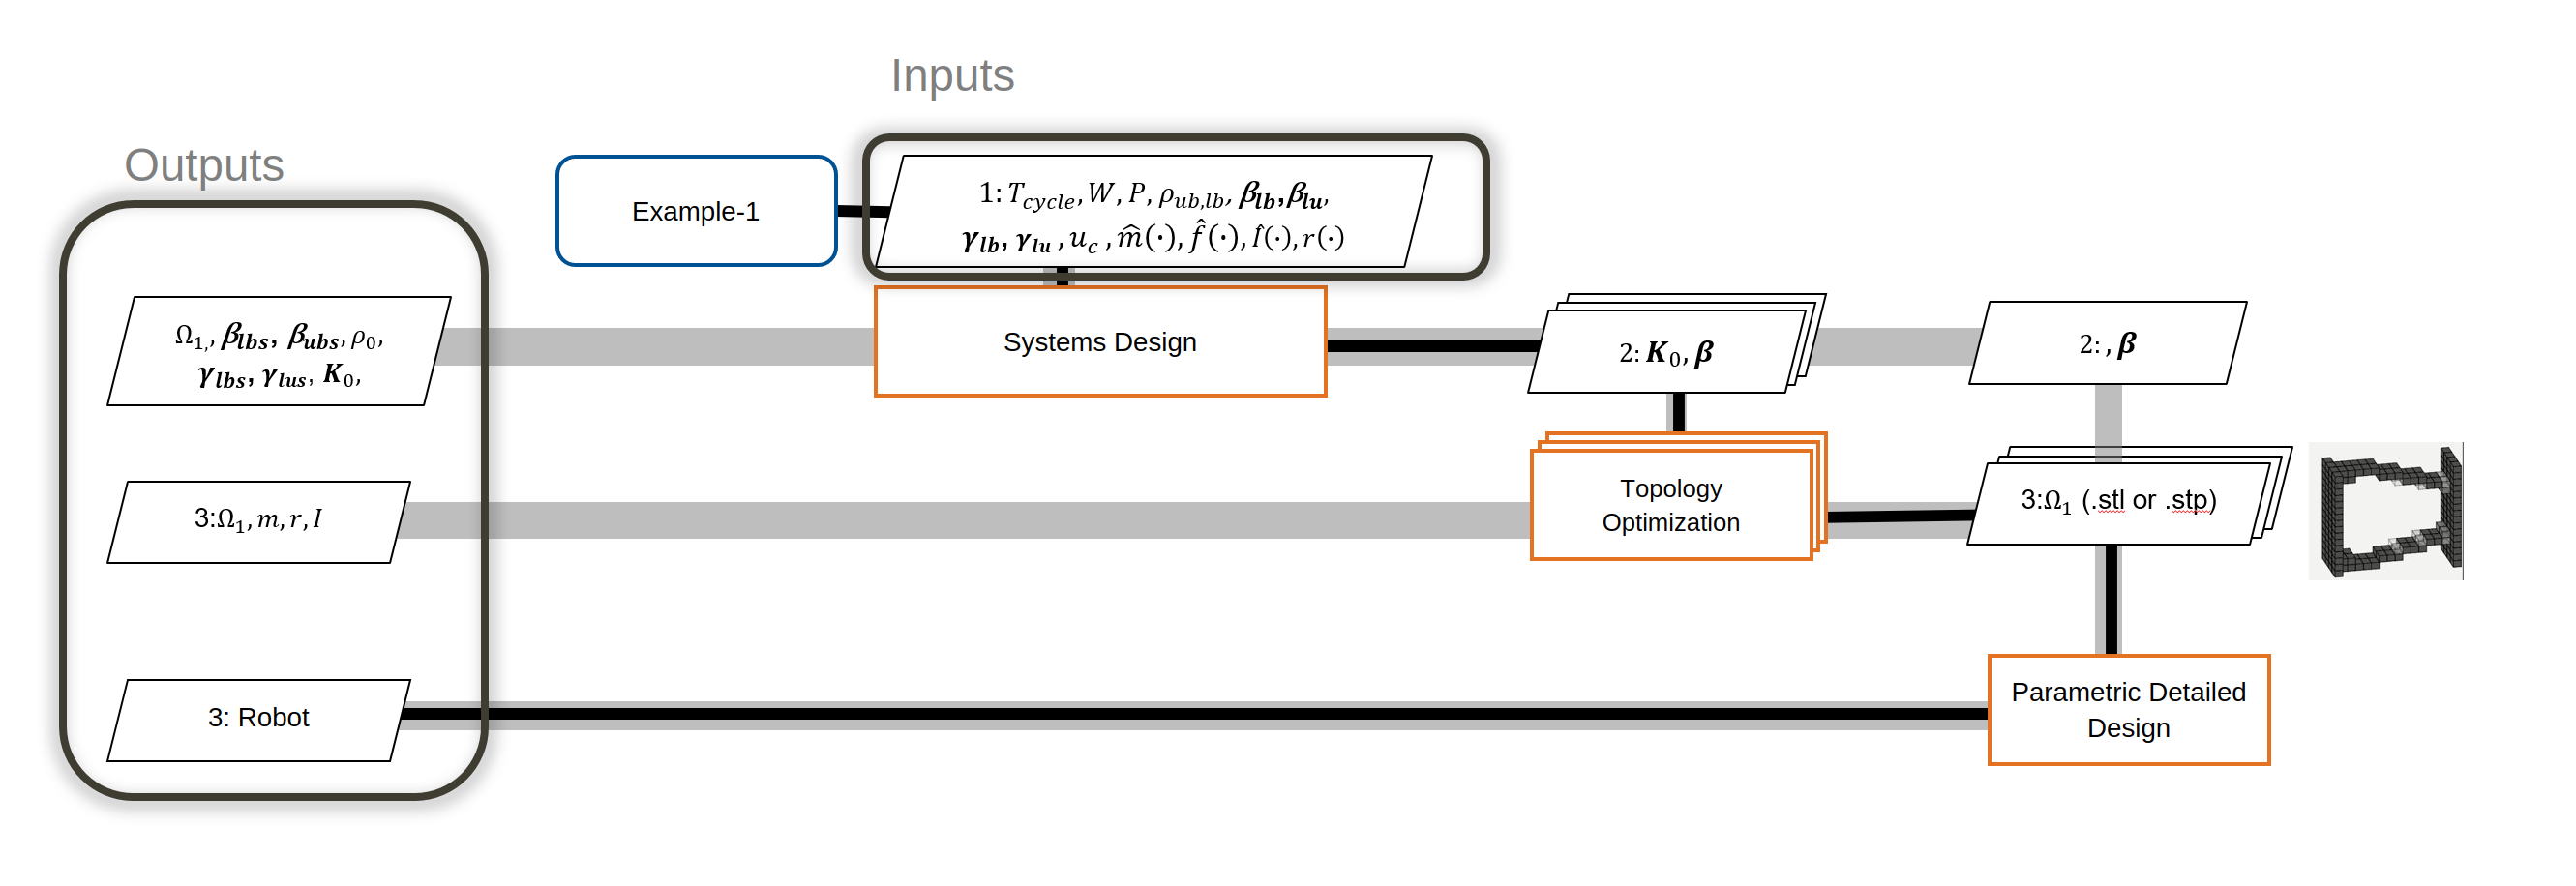
\includegraphics[scale=0.1]{xdsm-diva.png}
	\caption{XDSM of the design procedure of DIVA}
	\label{fig:xdsm}
\end{figure}

\begin{figure}[h]
	\centering
	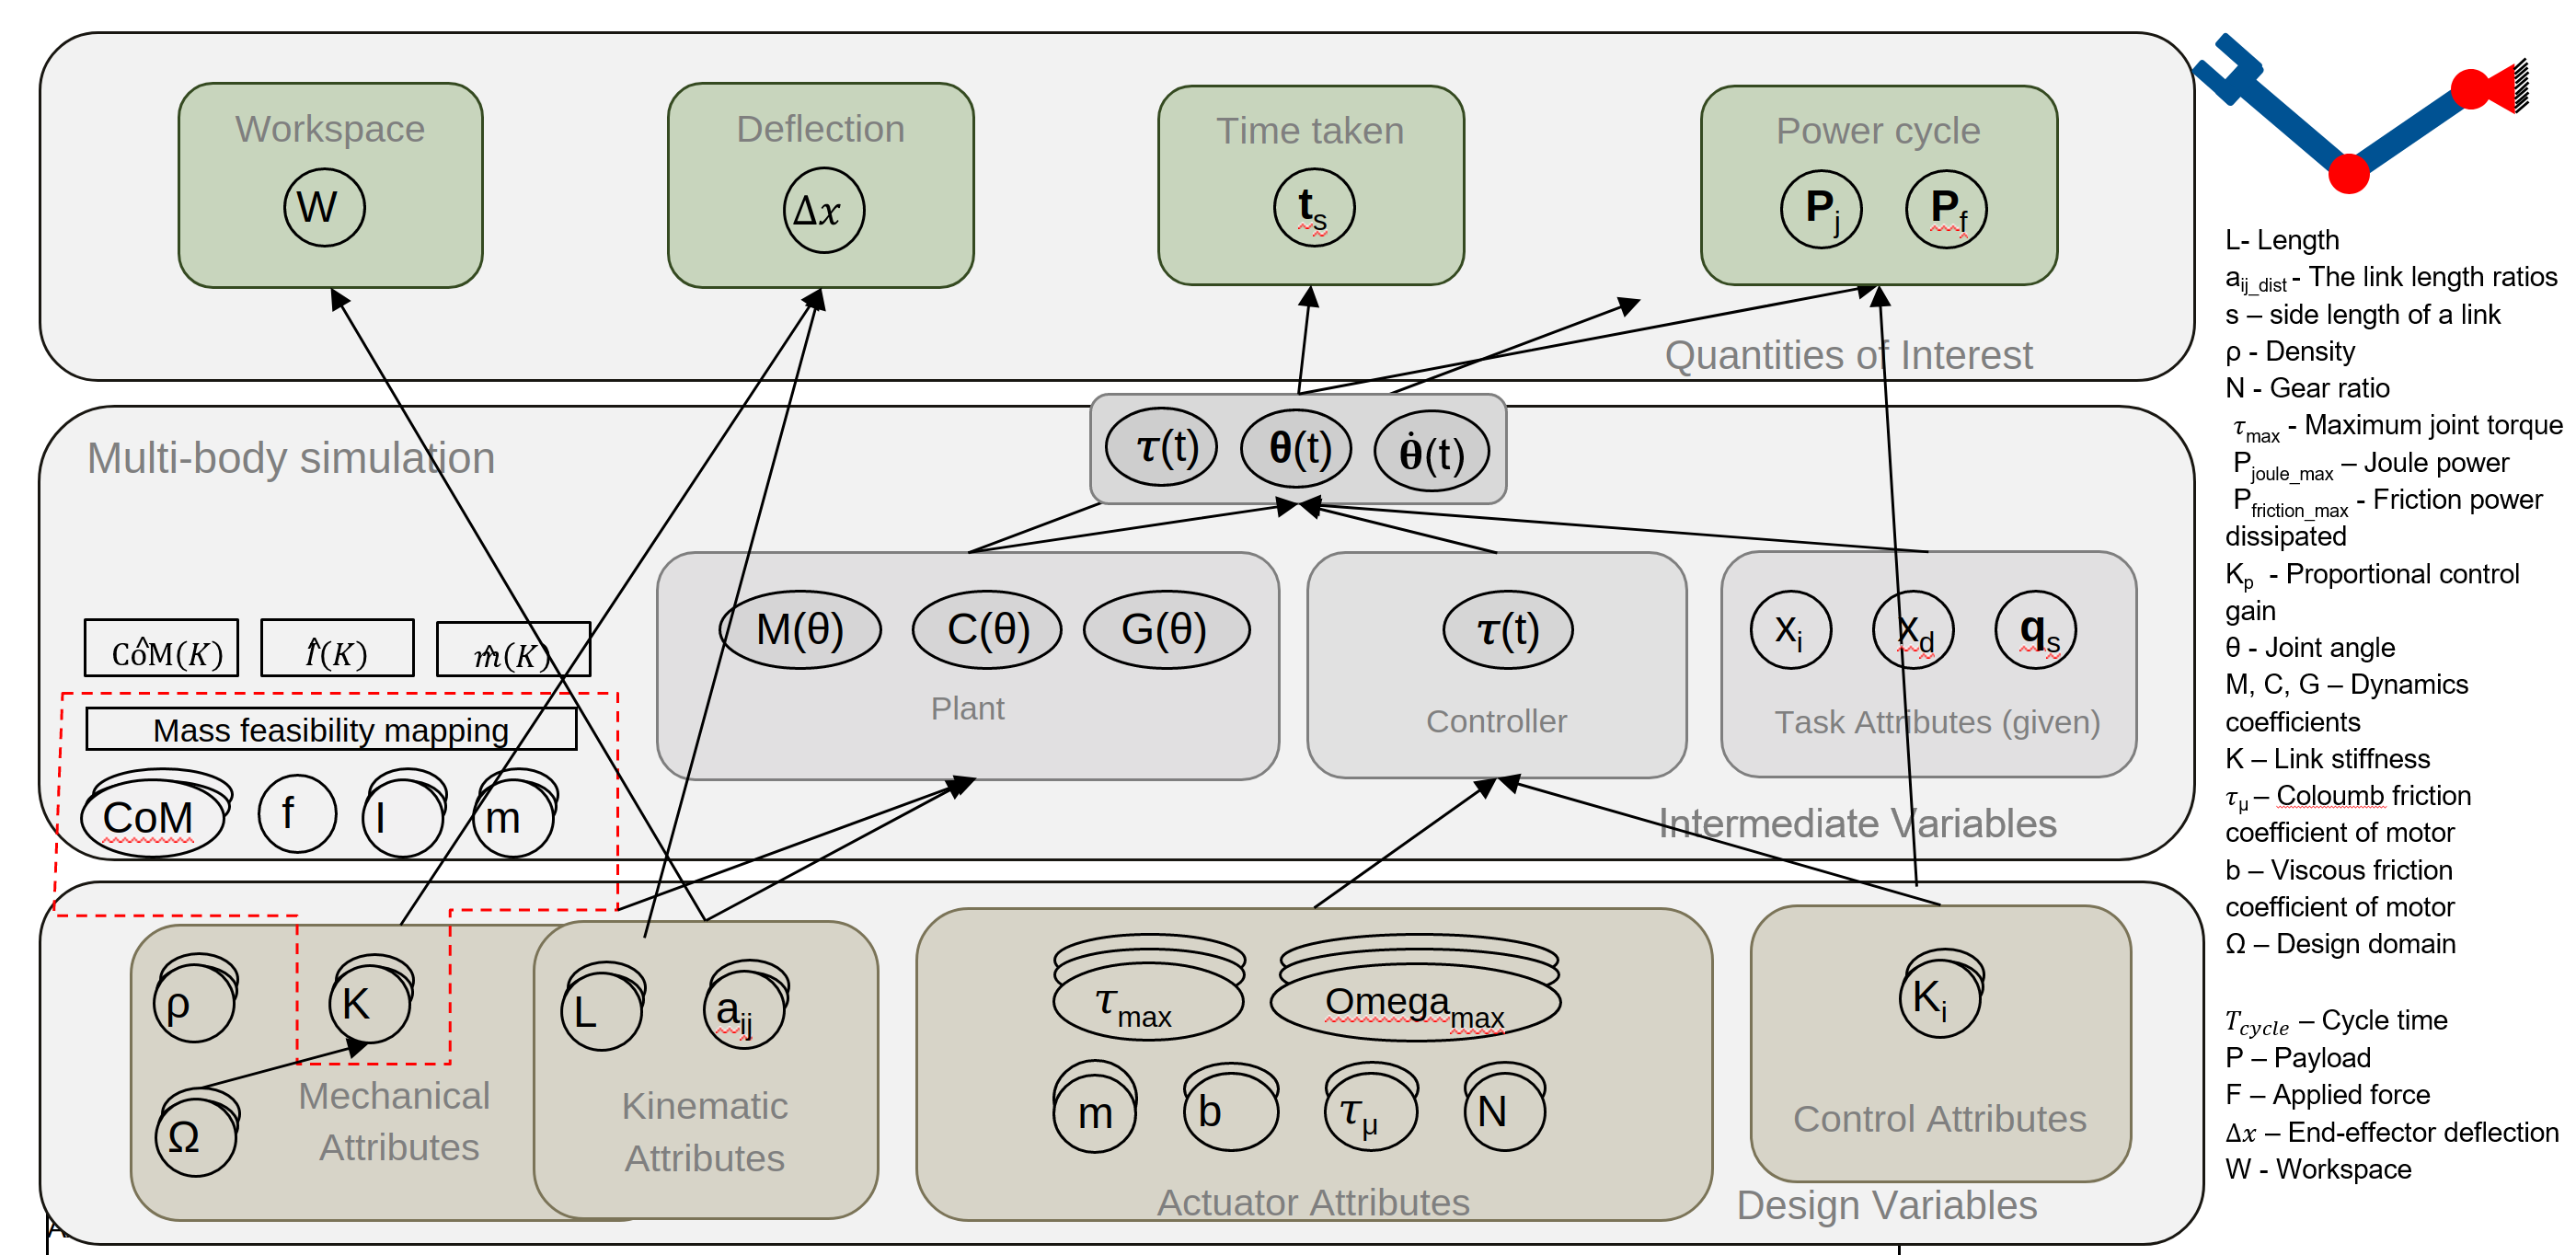
\includegraphics[scale=0.1]{adg-diva.png}
	\caption{ADG of the design procedure of DIVA\\\tbd{This remains almost the same, except make it look more professional in Windows and bring it back here}}
	\label{fig:adg}
\end{figure}

\subsection{Defining the bottom-up mappings}
\asc{Do we have paper-ready task definition that agrees with the NIST board and stuff? If not modify and also the use of more than one trajectory somehow? or justify the usage of a nominal trajectory and its capability to generalise over a range of positions. Or show it as something that can be adjusted post-process via solution spaces}

\asc{This includes the motor models, workspace definition, deflection?, heuristics, parametrising the URDF with link lengths with zero offset and motor mass and ratio to be within human dimensions}
\begin{figure}[h]
	\centering
	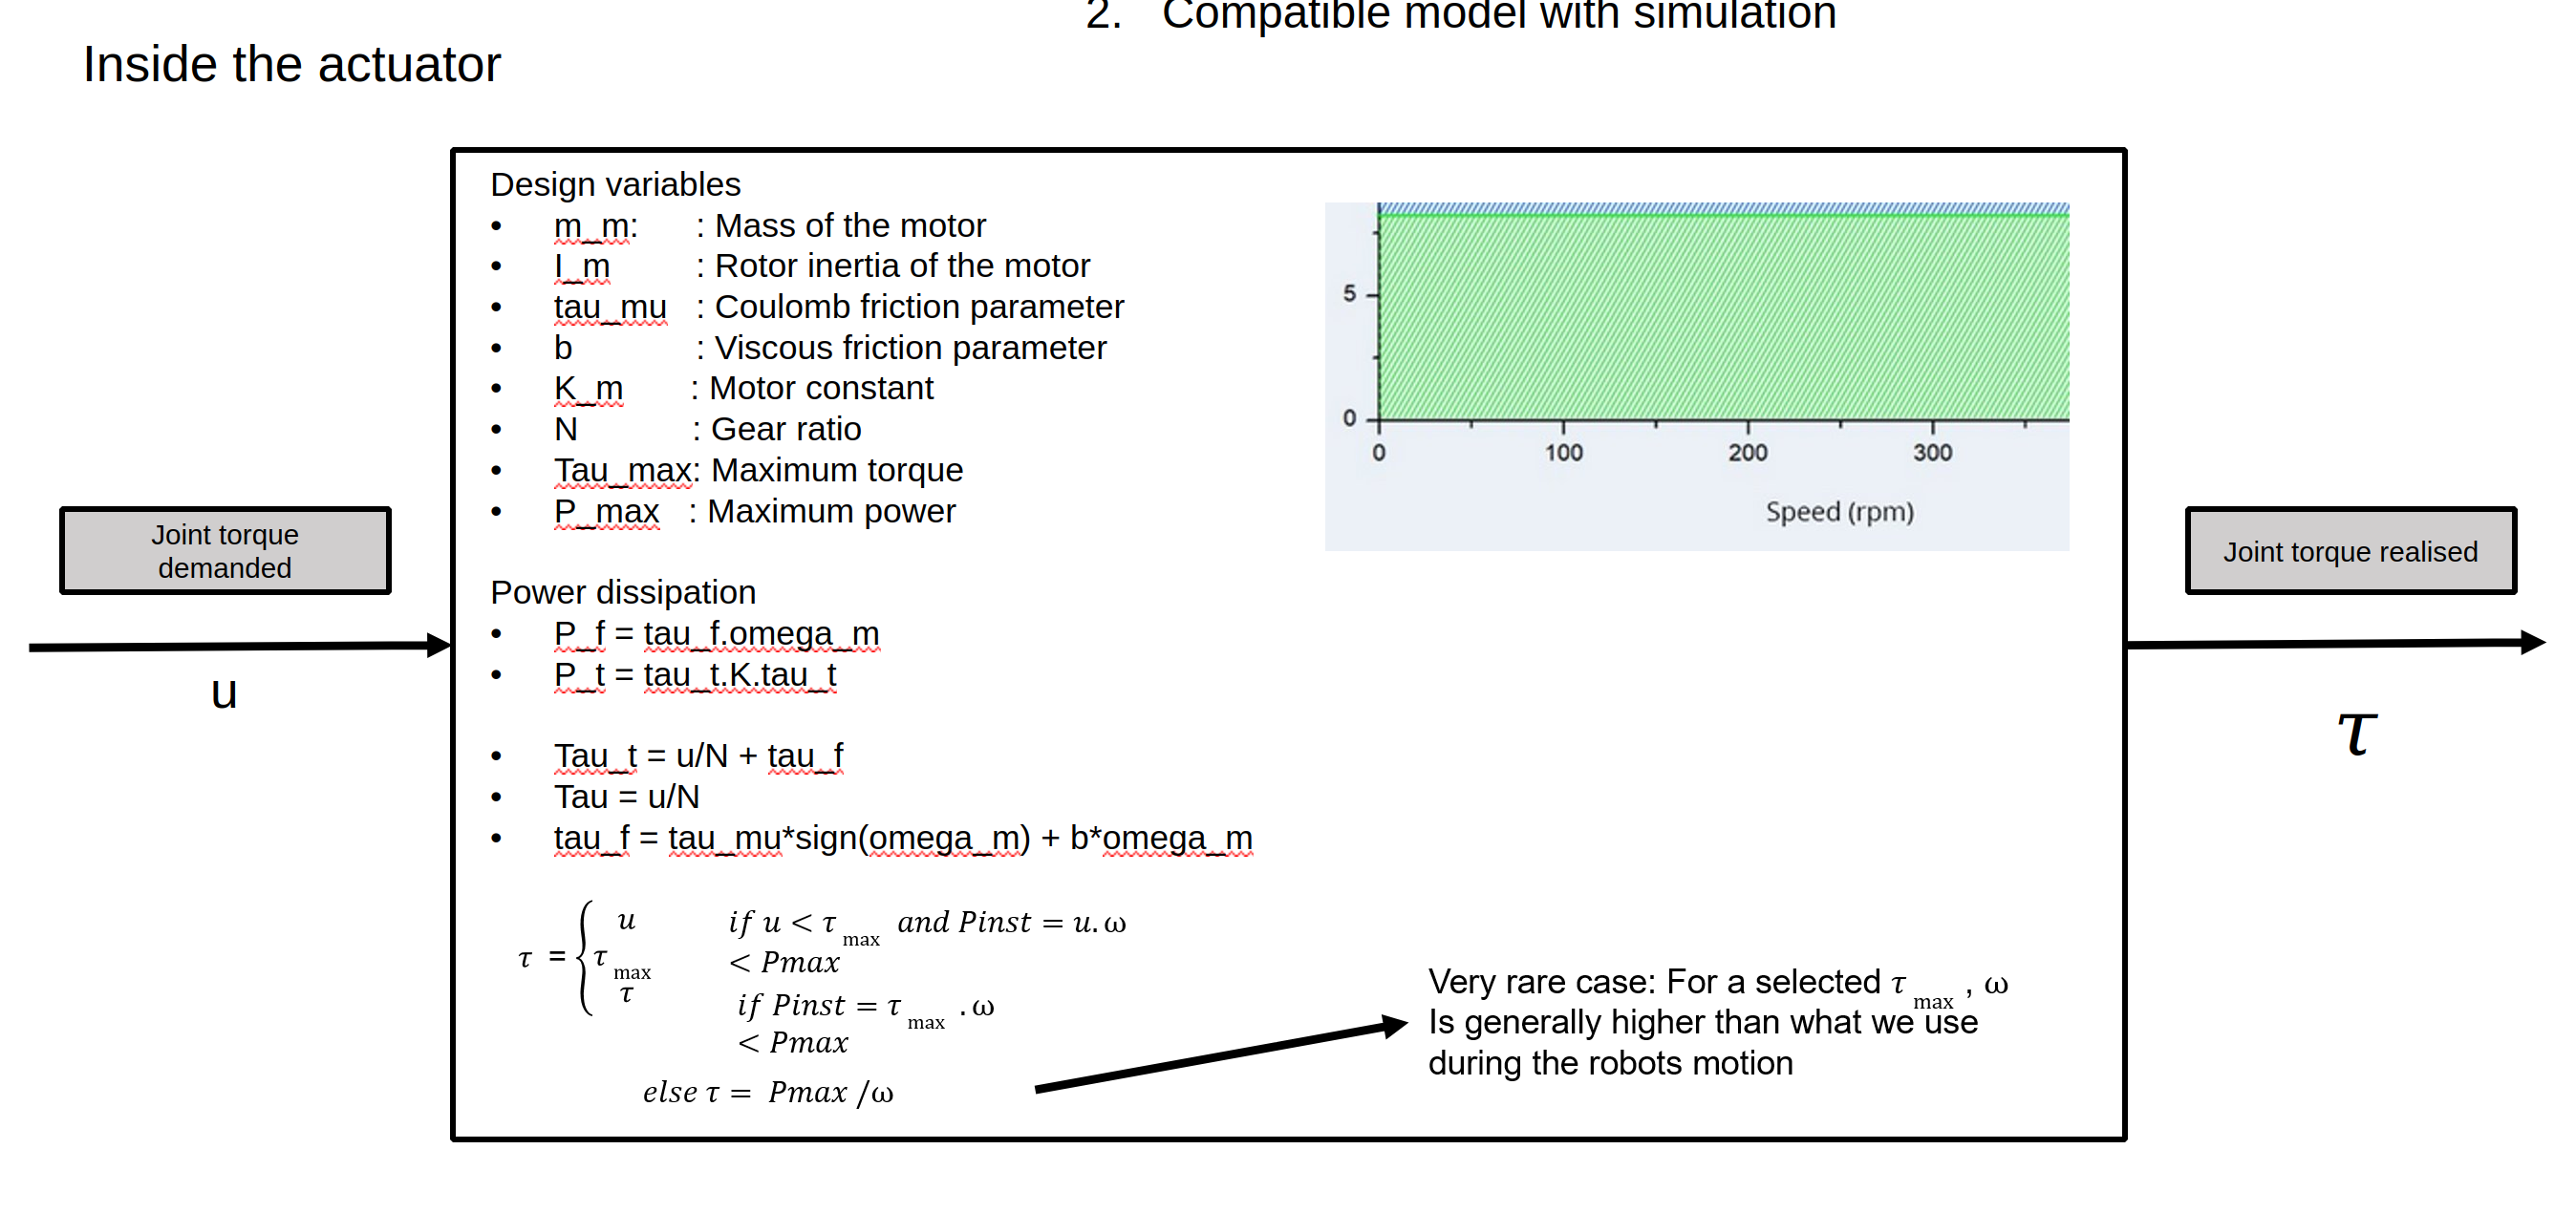
\includegraphics[scale=0.1]{motor-model-diva.png}
	\caption{Motor models used\\\tbd{This stays, but definitely not this form, maybe break it into different blocks}}
	\label{fig:motor_models}
\end{figure}

\subsection{Cost function components}
\asc{Explaining joule losses, workspace components, friction losses, payload and end-effector force applied}


\tbd{Now that we're clear on what kind of discussion and results we want to show, 
\begin{enumerate}
	\item Output design of the classical optimisation with heuristics
	\item Generate solution spaces around the unknown variables and the maximising boxes in the hardware space
	\item Back and forth between the designer and solution spaces to identify a physically feasible design
	\item Show a potential advantage by trading off a mechanical variable with respect to a hardware variable
	\item Show advantage of co-design: only optimising the mechanical variables
	\item Show advantage of co-design: only optimising the hardware parameters
	\item Show advantage of co-design: only optimising the control parameters
\end{enumerate}
}
\section{RESULTS}

\subsection{Task formulation}
\subsection{Optimisation framework}
\asc{Explain how URDFs are auto-created in drake and modified parameters and the usage of ODIO-URDF package, what kind of control we use for moving the robot between different points in space}
\subsection{Computing solution spaces}
\asc{Define how and what solution spaces are and how they have been used in the past etc.}
\subsection{Numerical results}
\asc{A logical thing to do is some ablation studies on how only parameters of mechanical then only control and then only hardware are optimised}
\subsection{Discussion}
\asc{How heuristics are limiting and the amount of energy savings and how the task generalises or the design procedure generalises over a bunch of tasks and robots}
\asc{Plots of joint torques showing how they barely solve the task as per top-down design strategy}
\asc{Trading off between different design variables and involving the mechanical design variables}

\section{CONCLUSIONS AND FUTURE WORK}
\asc{Usage of MPC or some other controllers or usage of a policy with a response surface/NN which can be differentiable through and solving the problem with gradients}

%%%%%%%%%%%%%%%%%%%%%%%%%%%%%%%%%%%%%%%%%%%%%%%%%%%%%%%%%%%%%%%%%%%%%%%%%%%%%%%%



%%%%%%%%%%%%%%%%%%%%%%%%%%%%%%%%%%%%%%%%%%%%%%%%%%%%%%%%%%%%%%%%%%%%%%%%%%%%%%%%


\newpage
%%%%%%%%%%%%%%%%%%%%%%%%%%%%%%%%%%%%%%%%%%%%%%%%%%%%%%%%%%%%%%%%%%%%%%%%%%%%%%%%
\section*{APPENDIX}

Appendixes should appear before the acknowledgment.

\section*{ACKNOWLEDGMENT}

The preferred spelling of the word  acknowledgment  in America is without an  e  after the  g . Avoid the stilted expression,  One of us (R. B. G.) thanks . . .   Instead, try  R. B. G. thanks . Put sponsor acknowledgments in the unnumbered footnote on the first page.


%%%%%%%%%%%%%%%%%%%%%%%%%%%%%%%%%%%%%%%%%%%%%%%%%%%%%%%%%%%%%%%%%%%%%%%%%%%%%%%%

References are important to the reader; therefore, each citation must be complete and correct. If at all possible, references should be commonly available publications.

\bibliographystyle{IEEEtran}
\bibliography{stewart}

\end{document}
